\documentclass{standalone}

\begin{document}

\begin{figure*}
  \caption{\label{fig:imgbuild}
    Illustration marking intermediary steps during the image forming process.
    The new image is first created that defaults to black.
    During execution, the \emph{apply\_lens} algorithm iterates through each pixel of the newly generated image and uses the passed lensing map to determine which pixel from the input should be placed at that location.}
  \begin{tikzpicture}[>=stealth,line width=3pt]
    \tikzset{every node/.style={inner sep=0pt}}
    \def\voffset{3.75cm}
    \def\hoffset{5cm}
    \node (in) at (-\hoffset,0pt)
      {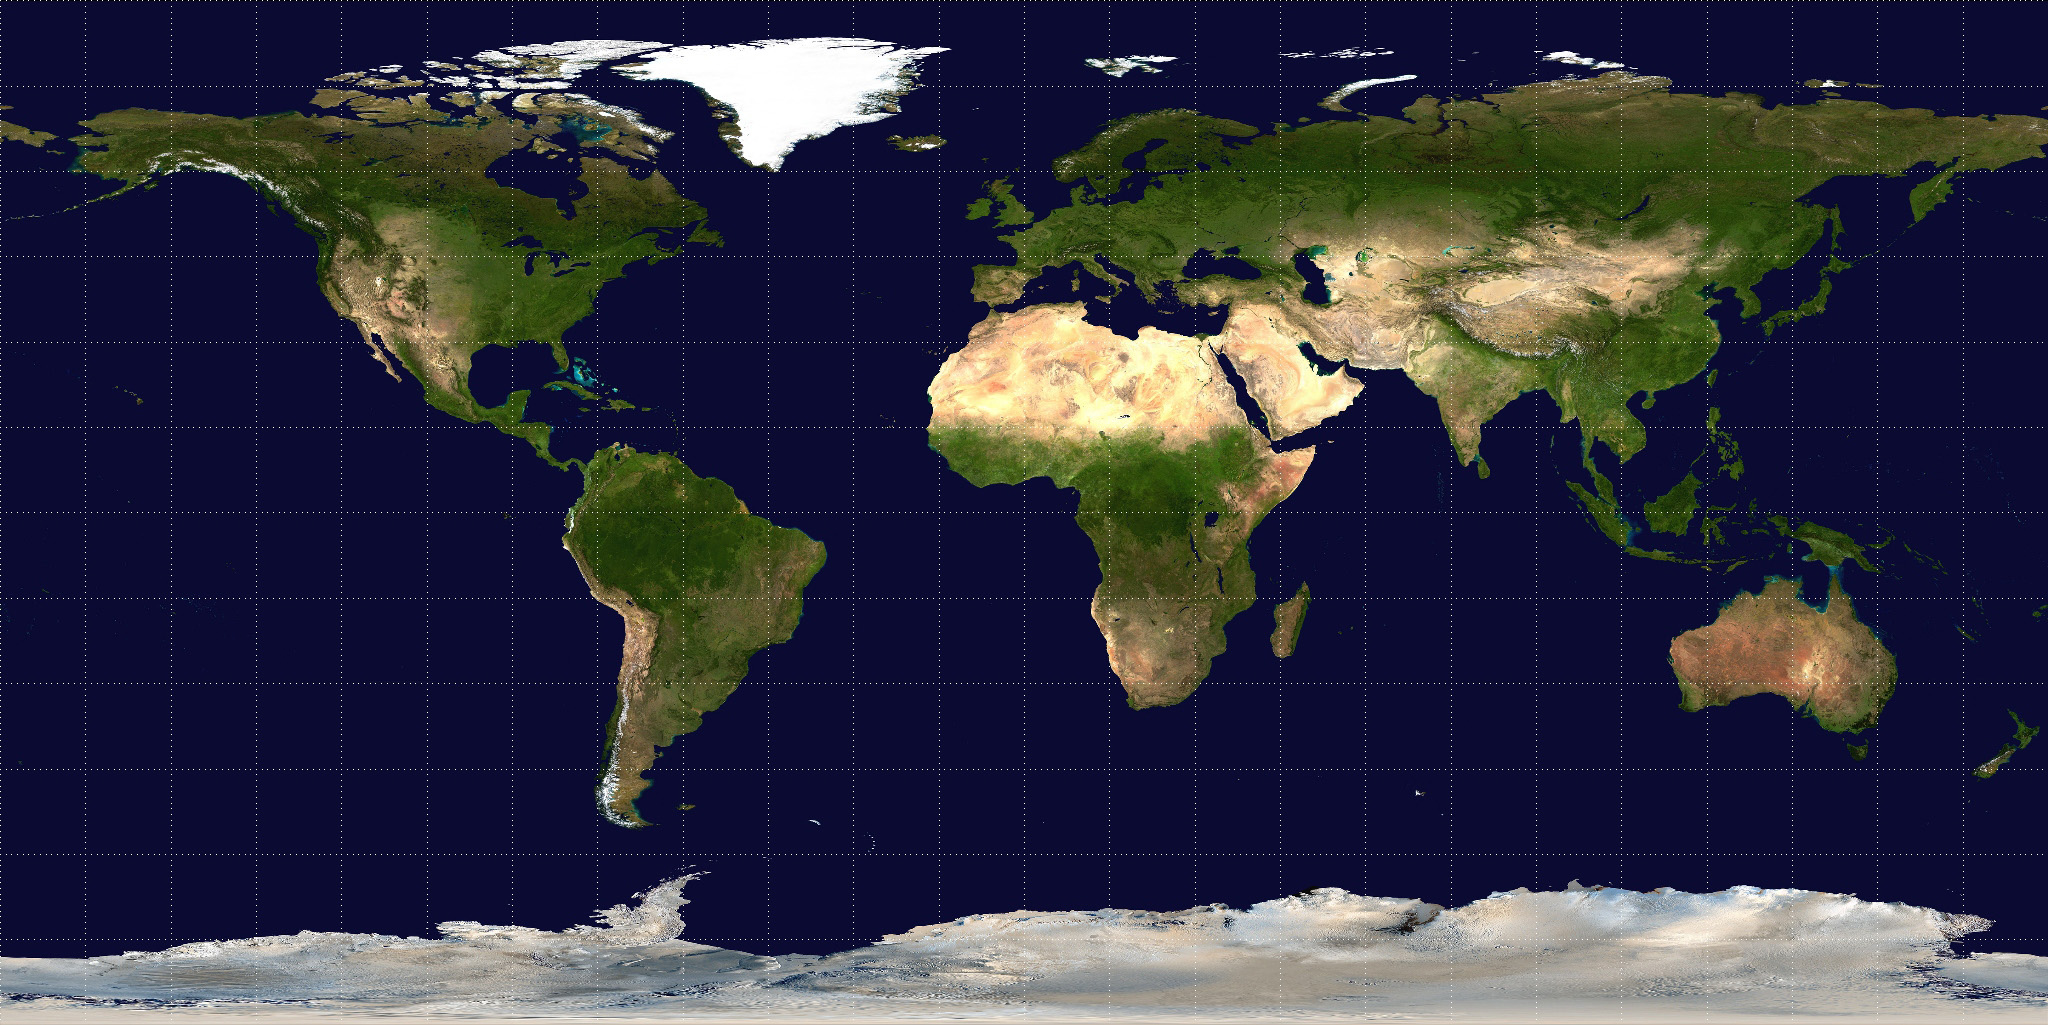
\includegraphics[width=.4\textwidth]{earth}};
    \node (out1) at (\hoffset,\voffset)
      {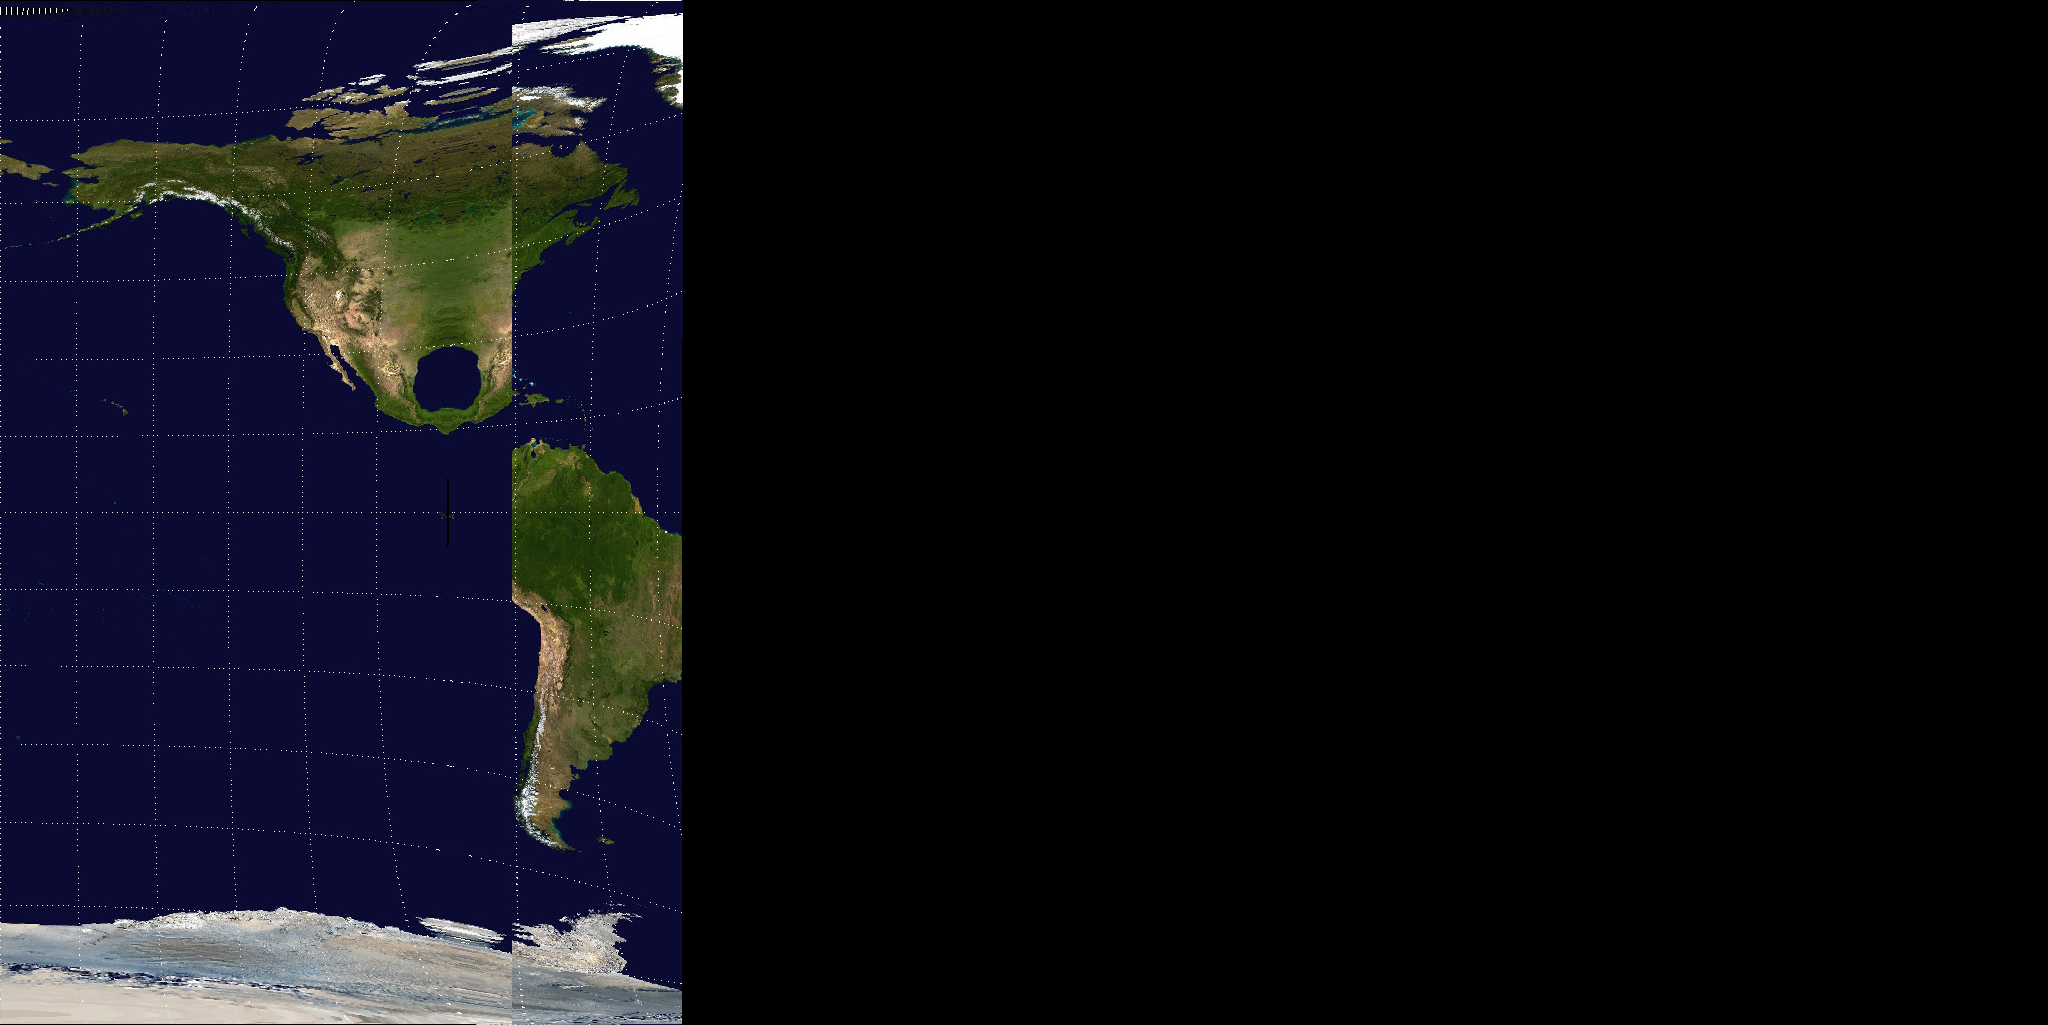
\includegraphics[width=.35\textwidth]{output_onethird}};
    \node (out2) at (\hoffset,0pt)
      {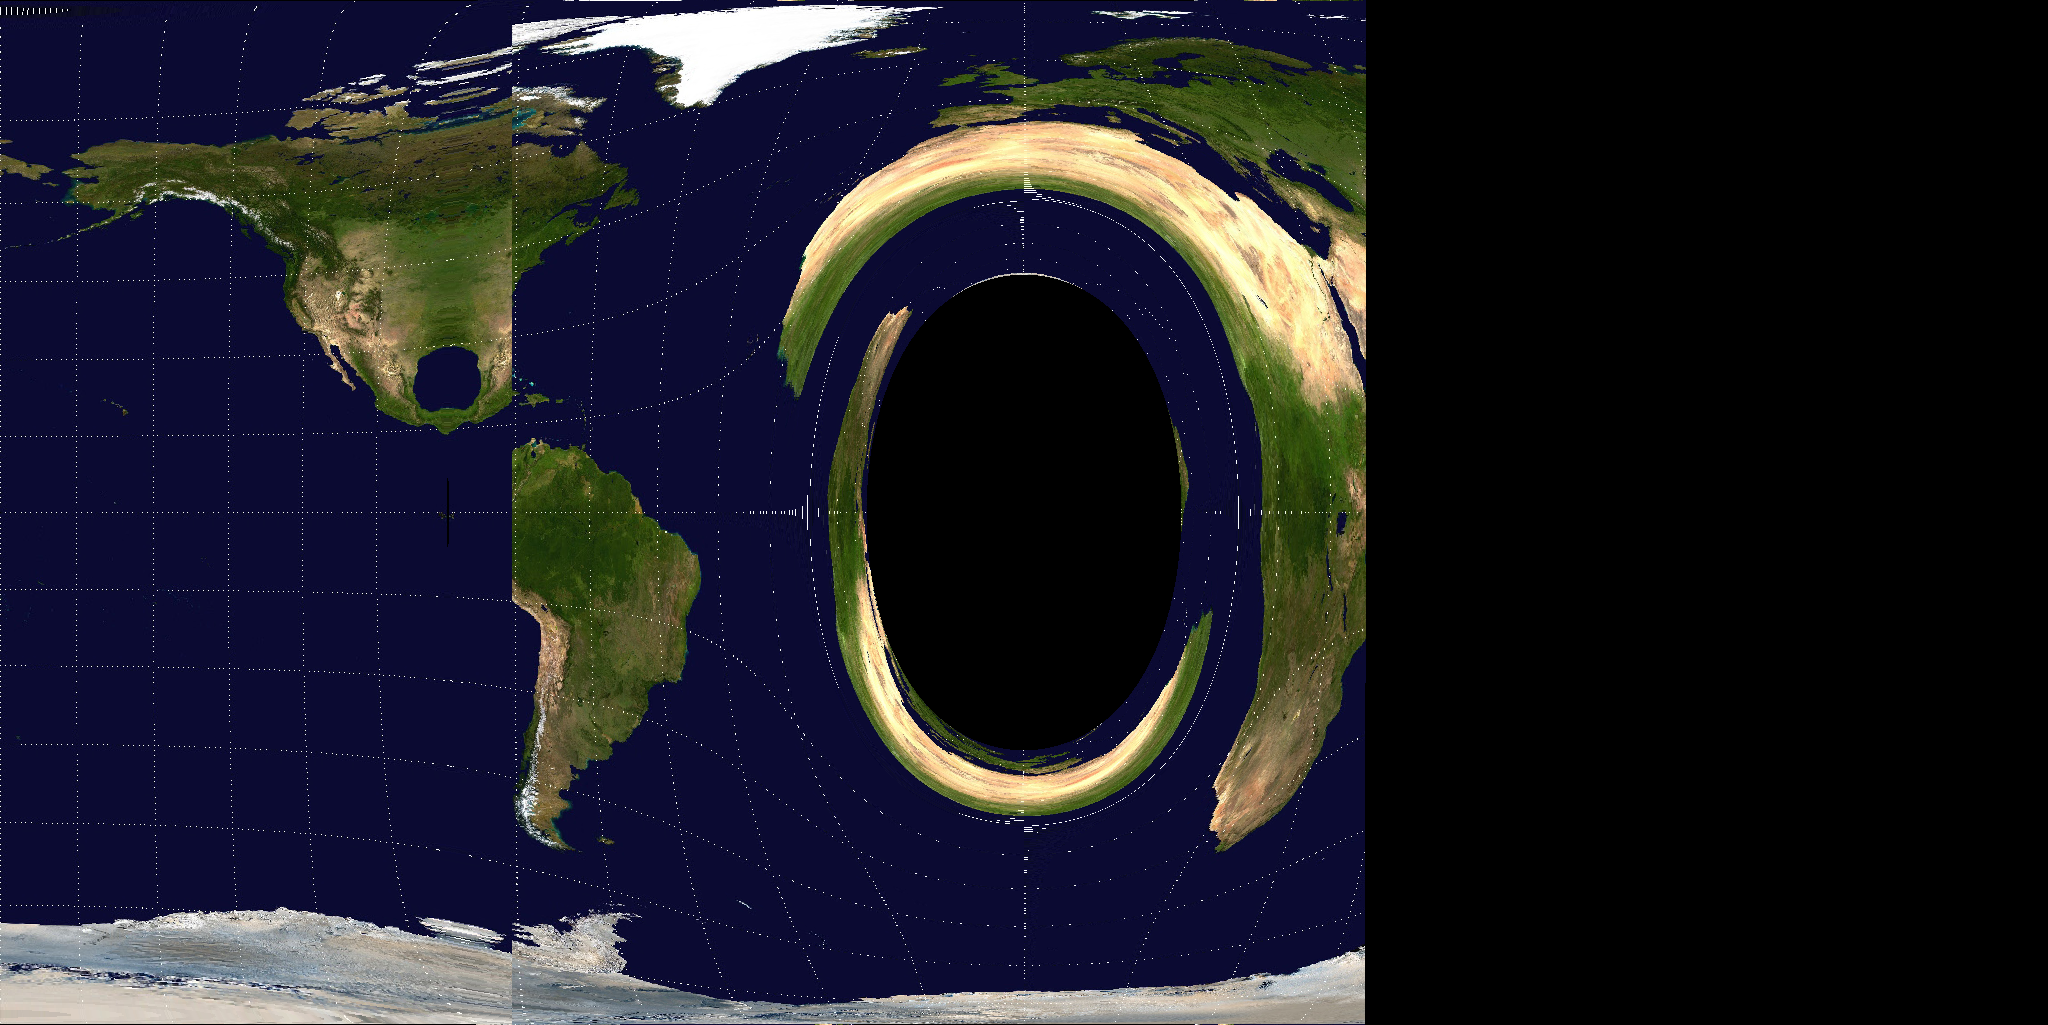
\includegraphics[width=.35\textwidth]{output_twothird}};
    \node (out3) at (\hoffset,-\voffset)
      {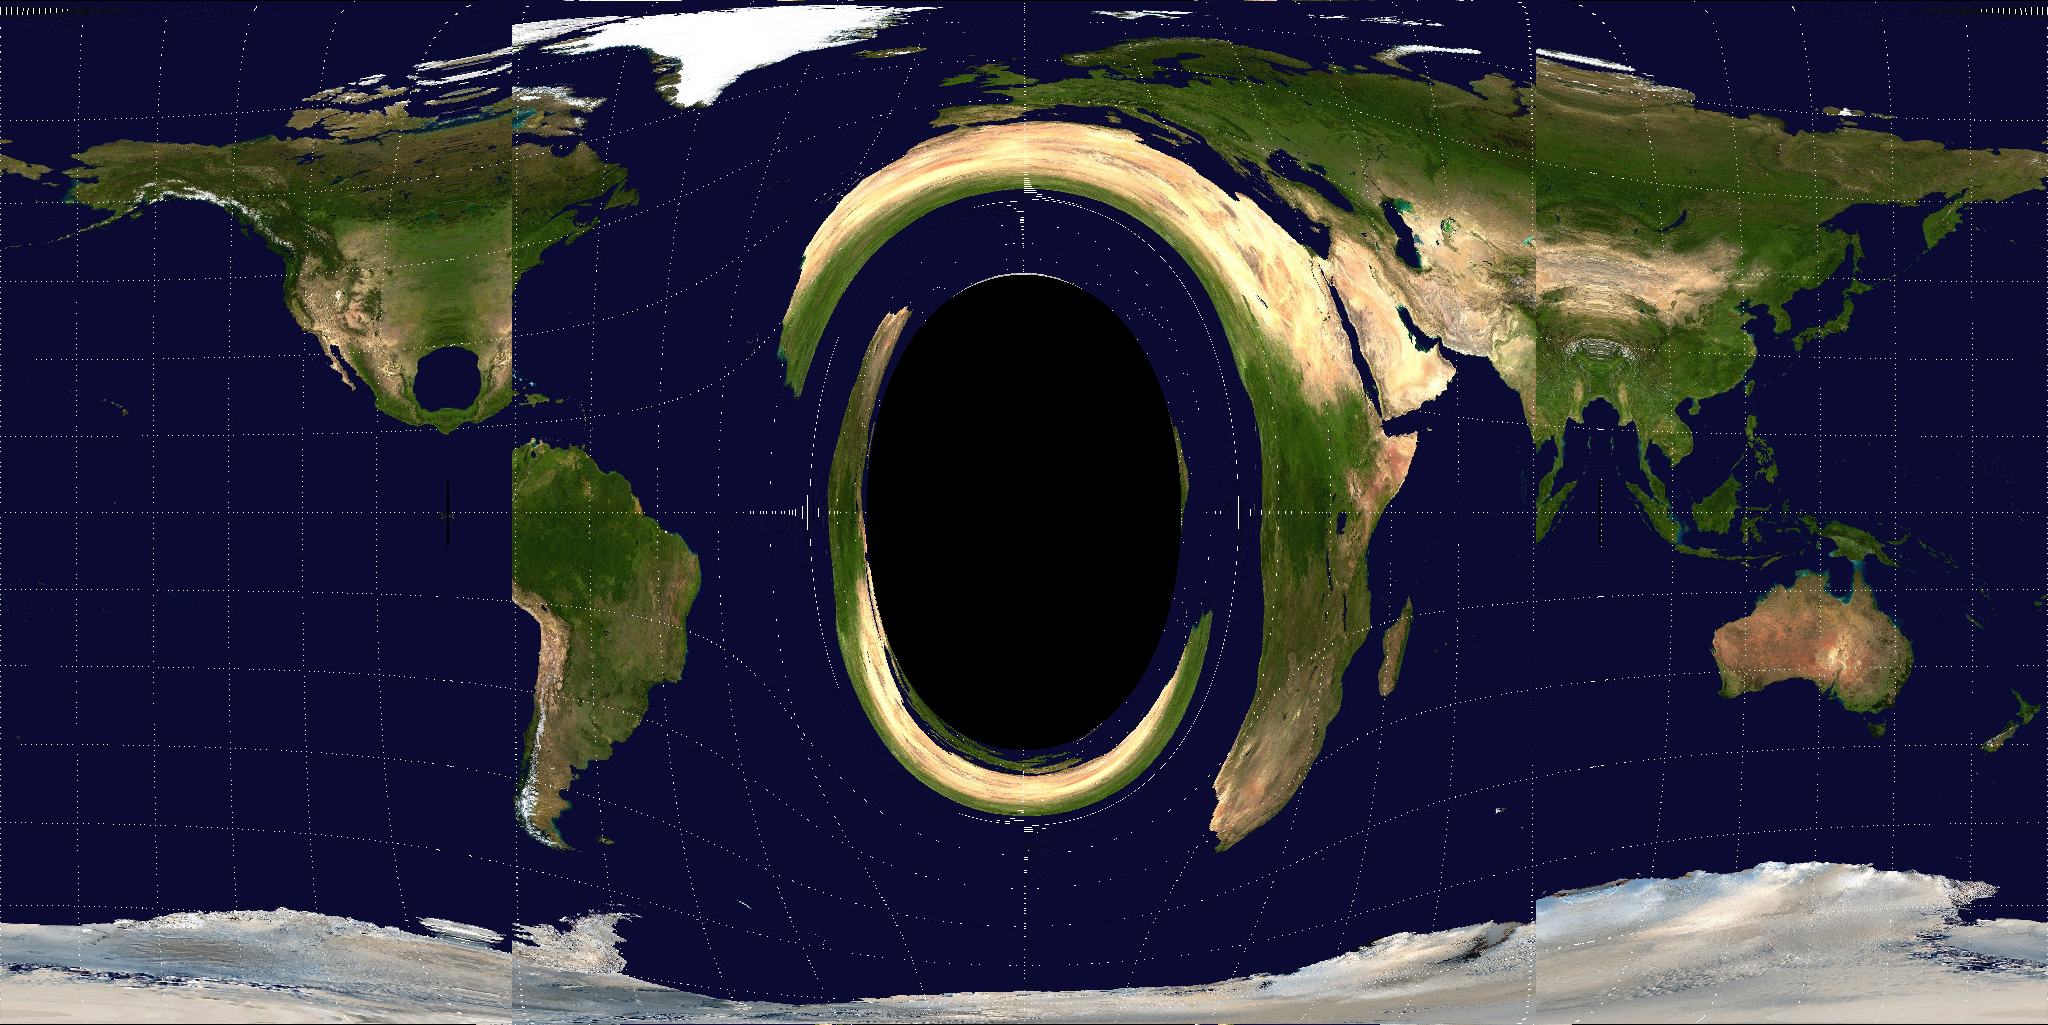
\includegraphics[width=.35\textwidth]{output_full}};
    \draw[->,shorten <=5mm,shorten >=5mm] (in) -- (out2);
    \draw[->] (out1) -- (out2);
    \draw[->] (out2) -- (out3);
  \end{tikzpicture}
\end{figure*}

\end{document}
